%***************************************PREAMBLE***************************************
\documentclass[a4paper,12pt]{article}

\usepackage[utf8]{inputenc}
\usepackage[margin=0.7in]{geometry}
\usepackage[T1]{fontenc}
\usepackage{graphicx}
\usepackage{float}
\usepackage{setspace}
\usepackage{appendix}
\usepackage{amsmath}
\usepackage{amssymb}
\usepackage{cite}
\usepackage{caption}
\usepackage{subcaption}


%***************************************DOCUMENT***************************************

\DeclareMathOperator*{\argmin}{\arg\!\min}
\DeclareMathOperator*{\argmax}{\arg\!\max}

\graphicspath{ {./images/} }
\setlength{\parindent}{0pt}

\begin{document}
	\fontfamily{ptm}\selectfont
	%%%%%%%%%%%%%%%%%%%%%%%%%%%%%%%%%%%%%%%COVERSHEET%%%%%%%%%%%%%%%%%%%%%%%%%%%%%%%%%%%%%%%
	\begin{titlepage}
		\setlength{\voffset}{-0.8in}
		\noindent \makebox[\textwidth]{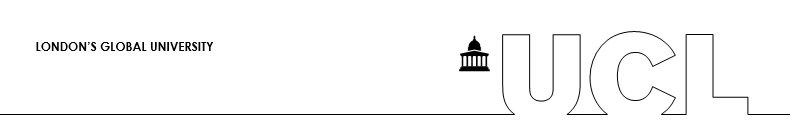
\includegraphics[width=1.2\textwidth]{Coversheet_Header.png}}
		
		\vspace{15mm}
		
		\begin{center}
			{\Huge \textbf{COMP0037 \\ \vspace{10mm} Report}}
			
			\vspace{8mm}
			
			\begin{spacing}{1.8}
				{\huge Planning in Uncertain Worlds}
			\end{spacing}
			
			
			\vspace{12mm}
			
			{\LARGE \textbf{Group AS}}
			
			\vspace{10mm}
			
			\begin{tabular}{ll}
				\underline{\textbf{Student Name}}  & \hspace{4mm} \underline{\textbf{Student number}} \vspace{2mm} \\
				Arundathi Shaji Shanthini & \hspace{4mm} 16018351 \\ 
				Dmitry Leyko & \hspace{4mm}  16021440\\ 
				Tharmetharan Balendran & \hspace{4mm} 17011729\\ 
			\end{tabular}
			
			\vspace{13mm}
			
			\begin{tabular}{ll}
				\textbf{Department:} &  Department of Electronic and Electrical Engineering\\ \vspace{3mm}
				\textbf{Submission Date:} &  28\textsuperscript{th} of April 2020
			\end{tabular}
		\end{center}
	\end{titlepage}
	%%%%%%%%%%%%%%%%%%%%%%%%%%%%%%%%%%%%%%
	
	\pagebreak
	
	\tableofcontents
	
	\pagebreak
	
	%%%%%%%%%%% PART 1 %%%%%%%%%%%%%%%%%
	\section{Policy Selection in a Dynamic Environment}
	\label{sec:policySelectionInADynamicEnvironment}
	
		\subsection{Policy Selection when Obstacle is Observed}
		\label{sec:policySelectionWhenObstacleIsObserved}
		
			\begin{figure}[H]
				\centering
				\begin{subfigure}{.4\textwidth}
					\centering
					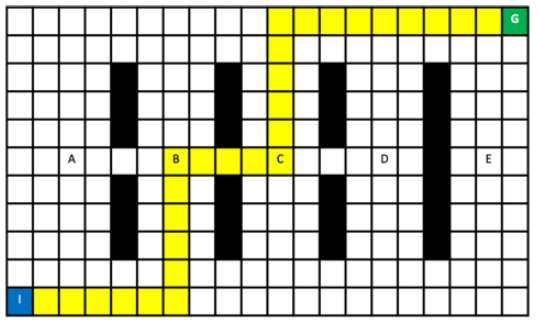
\includegraphics[width=\linewidth]{originalPlannedPath.png}
					\caption{The original planned path form I to G going through Aisle B and C.}
					\label{fig:originalPlannedPath}
				\end{subfigure}
				\begin{subfigure}{.4\textwidth}
					\centering
					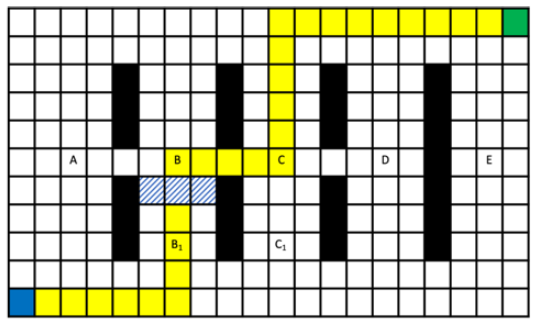
\includegraphics[width=\linewidth]{blockedAisleB.png}
					\caption{An obstacle in aisle B obstructs the planned path of the robot.}
					\label{fig:blockedAisleB}
				\end{subfigure}
				\caption{Illustration of case where robot observes an obstruction to it's planned path.}
				\label{fig:task1_1Figures}
			\end{figure}
			
			The scenario that we will be analysing is the case shown in Fig. \ref{fig:originalPlannedPath}. The robot is required to go from a cell $I$ to a cell $G$. These cells are marked blue and green in Fig. \ref{fig:originalPlannedPath} respectively. The figure also shows the original planned path that the robot computed going down aisle B. However, once the robot turns into aisle B it observes that the aisle is blocked. This observation is done at the point when the robot reaches the cell labelled $B_{1}$. At this point the robot can either decide to wait until the obstruction clears or it can re-plan a path. Once the robot observes the obstacle, the time the robot must wait for the obstacle to clear may be represented by the expression in Eq. (\ref{eqn:waitTime}). 
			
			\begin{equation}
			T=\frac{0.5}{\lambda_{B}}+\widetilde{T}
			\label{eqn:waitTime}
			\end{equation}
			
			The wait time is dependent on $\lambda_{B}$ and a random variable $\widetilde{T}$. The random variable $\widetilde{T}$ is sampled from a exponential distribution with a rate parameter of $2\lambda_{B}$. The probability density function (PDF) for $\widetilde{T}$ is shown in Eq. (\ref{eqn:waitTimePDF}). 
			
			\begin{equation}
			f(t) = 
			\begin{cases}
			\lambda e^{-\lambda t} & \quad t \geq 0 \\
			0 & \quad t < 0
			\end{cases}
			\label{eqn:waitTimePDF}
			\end{equation}
			where, the rate parameter $\lambda = 2\lambda_{B}$. 
			
			As previously mentioned, the robot has two options to choose from: to wait for the obstacle to clear, or to re-plan and execute the new path. The two are different policies the robot must choose from. We use the symbol $\pi$ to denote a policy. A policy is a mapping from the world state to an action the robot can execute.
			\\
			\\
			Let us assume that if the robot decides to wait the total path length (number of cells) will be $K_1$ while if the robot decides to re-plan and execute the total path length will be $K_2$. We let the quantity $K$ equal to the larger value between $K_1$ and $K_2$. Now we may write the policy for the robot to wait as $\pi_{K}^{1}$ and the policy for re-planning as $\pi_{K}^{2}$. These policies are padded correspondingly to produce actions $\textbf{u}_{K}^{1}$ and $\textbf{u}_{K}^{1}$ that are padded with zero-cost state preserving actions.
			\\
			\\
			To see which policy is better on average, we consider the expected value of the cost function for both cases. The case when policy $\pi_{K}^{1}$ is chosen is characterized by the inequality shown in Eq. (\ref{eqn:costExpectation}).
			
			\begin{equation}
			\mathbb{E}\left[L\left(\pi_{K}^{1}\right)\right] \leq \mathbb{E}\left[L\left(\pi_{K}^{2}\right)\right]
			\label{eqn:costExpectation}
			\end{equation}
			
			\begin{figure}[H]
				\centering
				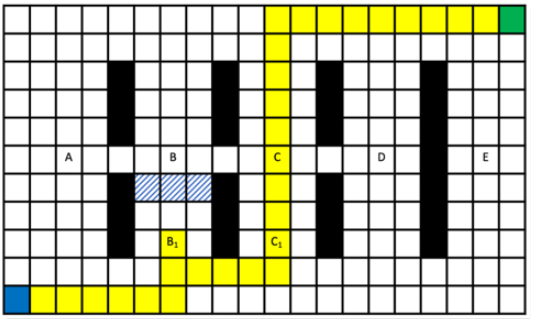
\includegraphics[scale=0.5]{images/replannedPathAisleB.png}
				\caption{The path for the re-plan policy $\pi_{K}^{2}$ which bypasses aisle B and goes down aisle C.}
				\label{fig:replannedPathAisleB}
			\end{figure}
			
			We can see from Fig. \ref{fig:originalPlannedPath} that the cost of the original planned path is given by the expression in Eq. (\ref{eqn:waitingPolicyCost}). In this equation, the terms $L_{XY}$ denote the cost of the shortest path between cell $X$ and cell $Y$. Additionally, the term $L_{W}$ represents the non-zero cost of the action $\boldsymbol{u}_w$. This action is state preserving (i.e. $\boldsymbol{x}_{k+1} = f(\boldsymbol{x}_k,\boldsymbol{u}_w) = \boldsymbol{x}_k$) and is used to represent the action of the robot waiting for one unit of time.
			
			\begin{equation}
			L\left(\pi_{K}^{1}\right) = L_{IB_{1}} + TL_W + L_{B_{1}B} + L_{BC} + L_{CG}
			\label{eqn:waitingPolicyCost}
			\end{equation}
			
			From Fig. \ref{fig:replannedPathAisleB} which shows the re-planned path, we can also see that the cost of this path is equal to the expression in Eq. (\ref{eqn:replanPolicyCost})
			
			\begin{equation}
			L\left(\pi_{K}^{2}\right) = L_{IB_{1}} + L_{B_{1}C_{1}} + L_{C_{1}C} + L_{CG}
			\label{eqn:replanPolicyCost}
			\end{equation}
			
			Substituting the expressions in Eq. (\ref{eqn:waitingPolicyCost}) and Eq. (\ref{eqn:replanPolicyCost}) into Eq. (\ref{eqn:costExpectation}). We obtain the inequality shown in Eq. (\ref{eqn:costExpectation1})
			
			\begin{equation}
			\begin{split}
			\mathbb{E}\left[L_{IB_{1}} + TL_W + L_{B_{1}B} + L_{BC} + L_{CG}\right] & \leq \mathbb{E}\left[L_{IB_{1}} + L_{B_{1}C_{1}} + L_{C_{1}C} + L_{CG}\right] \\
			L_{IB_{1}} + \mathbb{E}\left[T\right] L_W + L_{B_{1}B} + L_{BC} + L_{CG} & \leq L_{IB_{1}} + L_{B_{1}C_{1}} + L_{C_{1}C} + L_{CG} \\
			\mathbb{E}\left[T\right] & \leq \frac{L_{B_{1}C_{1}} + L_{C_{1}C} - L_{B_{1}B} - L_{BC}}{L_W}
			\end{split}
			\label{eqn:costExpectation1}
			\end{equation}
			
			The quantity $\mathbb{E}\left[T\right]$ is the expected value for the time the robot has to wait for the obstacle to clear. As we know the distribution that the variable is sampled from we can compute the expected value. The expected value for the time taken is given by the expression found in Eq. (\ref{eqn:waitTimeExpectation})
			
			\begin{equation}
			\begin{split}
				\mathbb{E}\left[T\right] & = \mathbb{E}\left[\frac{0.5}{\lambda_{B}}+\widetilde{T}\right] \\
				& = \frac{0.5}{\lambda_{B}} + \mathbb{E}\left[\widetilde{T}\right] \\
				& = \frac{0.5}{\lambda_{B}} + \int_{0}^{\infty}2\lambda_{B}te^{-2\lambda_{B}t} dt \\
				& = \frac{0.5}{\lambda_{B}} + 2\lambda_{B}\left[\left(t\right) \left(-\frac{1}{2\lambda_{B}}e^{-2\lambda_{B}t}\right) + \frac{1}{2\lambda_{B}} \int_{0}^{\infty}e^{-2\lambda_{B}t} dt \right]_{0}^{\infty} \\
				& = \frac{0.5}{\lambda_{B}} + 2\lambda_{B}\left[\left(t\right) \left(-\frac{1}{2\lambda_{B}}e^{-2\lambda_{B}t}\right) - \left(\frac{1}{2\lambda_{B}}\right)^2 e^{-2\lambda_{B}t} \right]_{0}^{\infty} \\
				& = \frac{0.5}{\lambda_{B}} - \left[te^{-2\lambda_{B}t} + \frac{1}{2\lambda_{B}} e^{-2\lambda_{B}t} \right]_{0}^{\infty} \\
				& = \frac{0.5}{\lambda_{B}} - (0 + 0 - 0 - \frac{1}{2\lambda_{B}}) = \frac{0.5}{\lambda_{B}} + \frac{1}{2\lambda_{B}} = \frac{1}{\lambda_{B}}
			\end{split}
			\label{eqn:waitTimeExpectation}
			\end{equation}
			
			Substituting the expression from Eq. (\ref{eqn:waitTimeExpectation}) into Eq. (\ref{eqn:costExpectation1}) we obtain the inequality in Eq. (\ref{eqn:lambdaInequality}). The right-hand side of the inequality in Eq. (\ref{eqn:lambdaInequality}) represents the smallest possible value for $\lambda_{B}$ for which the waiting policy $\pi_K^1$ is a better option than the re-plan policy $\pi_K^2$. The inequality also takes into consideration the constraint that $\lambda_{B} > 0$ and negates the solution when $\lambda_{B} < 0$.
			
			\begin{equation}
			\begin{split}
			\frac{1}{\lambda_{B}} & \leq \frac{L_{B_{1}C_{1}} + L_{C_{1}C} - L_{B_{1}B} - L_{BC}}{L_W} \\	
			\lambda_{B} & \geq \frac{L_W}{L_{B_{1}C_{1}} + L_{C_{1}C} - L_{B_{1}B} - L_{BC}}
			\end{split}
			\label{eqn:lambdaInequality}
			\end{equation}
		
		\subsection{Policy Selection at Start}
		\label{sec:policySelectionAtStart}
		
			\begin{figure}[H]
				\centering
				\begin{subfigure}{.4\textwidth}
					\centering
					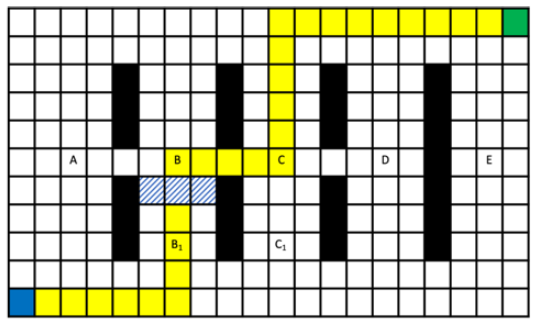
\includegraphics[width=\linewidth]{blockedAisleB.png}
					\caption{The scenario where the robot decides to go down Aisle B, encounters an obstacles and waits for it to clear.}
					\label{fig:plannedPathAisleB}
				\end{subfigure}
				\begin{subfigure}{.4\textwidth}
					\centering
					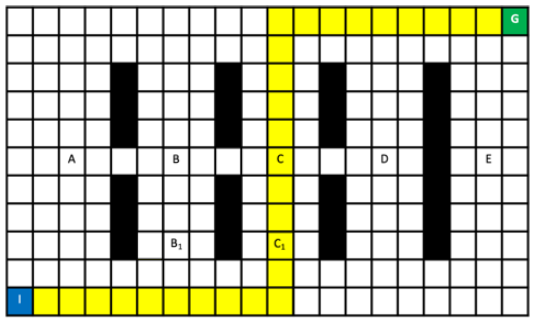
\includegraphics[width=\linewidth]{plannedPathAisleC.png}
					\caption{The scenario where the robot decides to avoid Aisle B completely due to the obstacle.}
					\label{fig:plannedPathAisleC}
				\end{subfigure}
				\caption{The different policies the robot can pick from at the beginning.}
				\label{fig:task1_2Figures}
			\end{figure}
			
			Instead of reacting to the obstacle as the robot observes it, the robot may also make a decision before it starts to move. The robot has knowledge of where the obstacles will be and the probability distribution for the wait time. Depending on the probabilities involved, the robot may decide to avoid the obstacle altogether instead of going the route with the obstacle and wait. In the case of the warehouse example with 5 aisles, and one obstacle in aisle B, the two policies are to choose to travel down aisle B and wait if an obstacle is present (illustrated in Fig. \ref{fig:plannedPathAisleB}) or to avoid aisle B and plan directly along aisle C (illustrated in Fig. \ref{fig:plannedPathAisleC}). By avoiding travelling down aisle B before replanning the robot avoids traversing the extra distance to the cell marked $B_1$ which makes this approach favorable.
			\\
			\\
			Similar to the approach in \S \ref{sec:policySelectionWhenObstacleIsObserved}, we may denote the policy that goes down aisle B as $\pi_{K}^{1}$ and the policy that goes down aisle C as $\pi_{K}^{2}$. We also consider the policy associated with choosing to go down aisle B and then replanning down aisle C as soon as the obstacle is observed. This policy will be represented as $\pi_{K}^{3}$. Once again these are padded with zero-cost state preserving actions so as to be of the same dimension. 
			\\
			\\
			Fig. \ref{fig:task1_2Figures} depicts the two possible paths that represent the two former policies. The three different policies and their costs are as follows:
			\begin{itemize}
				\item Policy $\pi_{K}^{1}$ : Drive down aisle B and wait for the obstacle to clear. The cost of this scenario is given by the expression in Eq. (\ref{eqn:waitPolicyCostStart}).
				\begin{equation}
				L(\pi_k^1) = L_{IB_1}+TL_W+L_{B_1B}+L_{BC}+L_{CG}
				\label{eqn:waitPolicyCostStart}
				\end{equation}
				\item Policy $\pi_{K}^{2}$ : Completely avoid aisle B and traverse directly to the goal via aisle C. It is known that no obstacle exists on this aisle. The cost for this policy is given in Eq. (\ref{eqn:aisleCPolicyCostStart}).
				\begin{equation}
				L(\pi_k^2) = L_{IC}+L_{CG}
				\label{eqn:aisleCPolicyCostStart}
				\end{equation}
				\item Policy $\pi_{K}^{3}$ : Choose to go down aisle B and then replan down aisle C as soon as the obstacle is observed. The cost of this policy is given in Eq. (\ref{eqn:replanPolicyCostStart})
				\begin{equation}
				L(\pi_k^2) = L_{IB_1}+L_{B_1C}+L_{CG}
				\label{eqn:replanPolicyCostStart}
				\end{equation}
			\end{itemize}
			
			Comparing the costs for policies $\pi_{K}^{2}$ and $\pi_{K}^{3}$ (given by Eq. (\ref{eqn:aisleCPolicyCostStart}) and Eq. (\ref{eqn:replanPolicyCostStart}) respectively), we can see that they only differ by only a few terms. Whereas $\pi_{K}^{2}$ goes directly down aisle C, $\pi_{K}^{3}$ first attempts to go down aisle B. This results in $\pi_{K}^{2}$ having the cost $L_{IC}$ to get to aisle C while $\pi_{K}^{2}$ has the cost $L_{IB_1}+L_{B_1C}$ to get to aisle C. As $L_{IC}$ is the cost of the best path, $L_{IC} \leq L_{IB_1}+L_{B_1C}$. Therefore we may ignore policy $\pi_{K}^{3}$ as the robot will always pick policy $\pi_{K}^{2}$ over policy $\pi_{K}^{3}$.
			\\
			\\
			As we are concerned with the average case scenario we compare the expected value of the loss function just as we did in section \ref{sec:policySelectionWhenObstacleIsObserved}. Policy $\pi_{K}^{2}$ will be chosen over policy $\pi_{K}^{1}$ if the expected value of it's cost is lower as shown by Eq. (\ref{eqn:expectationInequality}).
			
			\begin{equation}
			\mathbb{E}\left[L\left(\pi_{K}^{2}\right)\right] \leq \mathbb{E}\left[L\left(\pi_{K}^{1}\right)\right]
			\label{eqn:expectationInequality}
			\end{equation}
			
			Then, substituting the loss functions from Eq. (\ref{eqn:waitPolicyCostStart}) and (\ref{eqn:aisleCPolicyCostStart}) into the inequality in Eq. (\ref{eqn:expectationInequality}), we obtain the result shown in Eq. (\ref{eqn:expectationInequality1}).
			
			\begin{equation}
			\begin{split}
			\mathbb{E}[L_{IC}+L_{CG}] &\leq \mathbb{E}[L_{IB_1}+TL_W + L_{B_1B}+L_{BC}+L_{CG}] \\
			\mathbb{E}[T]L_W &\geq L_{IC}-L_{IB_1}-L_{B_1B}-L_{BC}\\
			\mathbb{E}[T] &\geq \frac{L_{IC}-L_{IB_1}-L_{B_1B}-L_{BC}}{L_W}
			\end{split}
			\label{eqn:expectationInequality1}
			\end{equation}
			
			By substituting the expected value for $T$ found in Eq. (\ref{eqn:waitTimeExpectation}) we obtain a constraint for $\lambda_B$ as shown in Eq. (\ref{eqn:constraintPlanAtStart}). The right hand side of the final inequality in Eq. (\ref{eqn:constraintPlanAtStart}) represents the largest value for $\lambda_B$ for which the robot will decide to go directly down aisle C avoiding aisle B. Once again the sultions for $\lambda_B < 0$ have been ignored. 
			
			\begin{equation}
			\begin{split}
			\frac{1}{\lambda_B} &\geq \frac{L_{IC}-L_{IB_1}-L_{B_1B}-L_{BC}}{L_W}\\
			\lambda_B &\leq \frac{L_W}{L_{IC}-L_{IB_1}-L_{B_1B}-L_{BC}}
			\end{split}
			\label{eqn:constraintPlanAtStart}
			\end{equation}
		
		\subsection{Considering the Probability of the Obstacle Being Present}
		
			In reality, the obstacle would not be present there all the time. This can be taken into account using a probability, say $p_B$ associated with the scenario that the obstacle is present\footnote{This means that the probability that the obstacle is absent can be given by $ (1-p_B) $}. The mean wait time in the case the obstacle is present has been derived in Eq. (\ref{eqn:waitTimeExpectation}). In the case the obstacle isn't present, the robot does not have wait and therefore the mean wait time is 0. By taking a sum of these wait times weighted by their probabilities of occurring we obtain the expected wait time that takes into consideration the probability of the obstacle being present as shown below in Eq. (\ref{eqn:expectedWaitTimeProbability}):
						
			\begin{equation}
			\begin{split}
				\mathbb{E}_B[T] &= p_B \cdot \mathbb{E}[T] + \left(1 - p_{B}\right) \cdot \left(0\right) \\
				&= p_B \cdot \frac{1}{\lambda_B} = \frac{p_B}{\lambda_B}
			\end{split}
			\label{eqn:expectedWaitTimeProbability}
			\end{equation}
			
			where, $\mathbb{E}[T]$ is expected time to wait given the obstacle in aisle B exist and it is given by Eq. \ref{eqn:costExpectation1}
			
			Given Eq. (\ref{eqn:expectedWaitTimeProbability}) we may reconsider Eq. (\ref{eqn:expectationInequality1}) and substitute this new value for the expected wait time:
			
			\begin{equation}
			\begin{split}
				\mathbb{E}_{B}[T] &\geq \frac{L_{IC}-L_{IB_1}-L_{B_1B}-L_{BC}}{L_W} \\
				\frac{p_B}{\lambda_B} &\geq \frac{L_{IC}-L_{IB_1}-L_{B_1B}-L_{BC}}{L_W}
			\end{split}
			\label{eqn:probabilityInequality1}
			\end{equation}
		
			Assuming that the rate parameter $\lambda_B$ is constant, we may arrive at the equation shown in Eq. (\ref{eqn:probabilityConstraint}).
			
			\begin{equation}
				p_B \geq \frac{\lambda_B\left(L_{IC}-L_{IB_1}-L_{B_1B}-L_{BC}\right)}{L_W}
			\label{eqn:probabilityConstraint}
			\end{equation}
		
			It should be noted however that this was the inequality to choose the policy to plan straight through aisle C. Therefore the R.H.S of the inequality in Eq. (\ref{eqn:probabilityConstraint}) represents the value for $p_B$ below which the robot will attempt to drive down aisle B first. 
		
		\subsection{Considering Multiple Obstacles}
		
			Let us now assume that both aisles B and C have obstacles on them. The wait time for the obstacle in aisle B to clear is sampled from the distribution outlined in Eq. (\ref{eqn:waitTime}). The probability of the obstacle in aisle B being present is once again given as $p_B$. Similarly the obstacle in aisle C has an identical wait time distribution as the obstacle in aisle B but with a characterizing parameter of $\lambda_C$. The probability of this obstacle being present is given by the probability $p_C$. Following this, the expected wait times for obstacle B and obstacle C are as follows:
			
			\begin{equation}
			\begin{split}
				\mathbb{E}_{B}[T] &= \frac{p_B}{\lambda_B} \\
				\mathbb{E}_{C}[T] &= \frac{p_C}{\lambda_C} \\
			\end{split}
			\label{eqn:expectedWaitTimeBC}
			\end{equation}
			
			The robot has the same start and goal cells as described in \S \ref{sec:policySelectionWhenObstacleIsObserved}. Given that the robot chooses a policy at the beginning, there are 6 different key scenarios that are worth considering:
			
			\begin{itemize}
				\item Policy $\pi_{K}^{1}$ : The robot goes down aisle B and observes an obstacle. It then decides to wait for the obstacle to clear. The expected cost for this policy is given by:
					\begin{equation}
						\mathbb{E}\left[L\left(\pi_{K}^{1}\right)\right] = L_{IB_1} + \mathbb{E}_{B}\left[T\right]L_W + L_{B_1B} + L_{BC} + L_{CG}
					\label{eqn:policyOneCost}
					\end{equation}
					
				\item Policy $\pi_{K}^{2}$ : The robot goes down aisle B and observes an obstacle so re-plans down aisle C. While travelling down aisle C it observes another obstacle and waits for it to clear before continuing to the goal. The expected cost for this policy is given by:
					\begin{equation}
						\mathbb{E}\left[L\left(\pi_{K}^{2}\right)\right] = L_{IB_1} + L_{B_1C_1} + \mathbb{E}_{C}\left[T\right]L_W + L_{C_1C} + L_{CG}
					\label{eqn:policyTwoCost}
					\end{equation}
				
				\item Policy $\pi_{K}^{3}$ : The robot goes down aisle B and observes an obstacle so re-plans down aisle C. While travelling down aisle C it observes another obstacles so it re-plans down aisle D which is known to have no obstacles. The expected cost for this policy is given by:
					\begin{equation}
						\mathbb{E}\left[L\left(\pi_{K}^{3}\right)\right] = L\left(\pi_{K}^{3}\right) = L_{IB_1} + L_{B_1C_1} + L_{C_1} + L_{DG}
					\label{eqn:policyThreeCost}
					\end{equation}
					
				\item Policy $\pi_{K}^{4}$ : The robot goes down aisle C and observes an obstacle so it waits for the obstacle to clear before continuing to the goal. The expected cost for this policy is given by:
					\begin{equation}
						\mathbb{E}\left[L\left(\pi_{K}^{4}\right)\right] = L_{IC_1} + \mathbb{E}_{C}\left[T\right]L_W + L_{C_1C} + L_{CG}
					\label{eqn:policyFourCost}
					\end{equation}
					
				\item Policy $\pi_{K}^{5}$ : The robot goes down aisle C and observes an obstacle so it re-plans down aisle D which is known to have no obstacles. The expected cost for this policy is given by:
					\begin{equation}
						\mathbb{E}\left[L\left(\pi_{K}^{5}\right)\right] = L\left(\pi_{K}^{5}\right) = L_{IC_1} + L_{C_1D} + L_{DG}
					\label{eqn:policyFiveCost}
					\end{equation}
				
				\item Policy $\pi_{K}^{6}$ : The robot directly goes down aisle D which is known to have no obstacles and avoids both aisles B and C. The expected cost for this policy is given by:
					\begin{equation}
						\mathbb{E}\left[L\left(\pi_{K}^{6}\right)\right] = L\left(\pi_{K}^{6}\right) = L_{ID} + L_{DG}
					\label{eqn:policySixCost}
					\end{equation}
			\end{itemize}
		
			We ignore the case of going down aisle A and aisle E as these will inherently have a larger path length due to the topology of the example scenario. Additionally back-tracking of aisles is also ignored (e.g. going from aisle C back to aisle B) as this would also have larger costs than those considered above.
			\\
			\\
			We are given that the robot chooses policy $\pi_{K}^{6}$ by going straight down aisle D. This suggests that the expected cost of this policy is lower than any other policy available to the robot as suggested by Eq. (\ref{eqn:minimumExpectation})
			
			\begin{equation}
				\mathbb{E}\left[L\left(\pi_{K}^{6}\right)\right] = \min_{n=1,\dots,6} \mathbb{E}\left[L\left(\pi_{K}^{n}\right)\right]
			\label{eqn:minimumExpectation}
			\end{equation}
	
			We can see that some of these policies have common terms. For example we may have a look at policies $\pi_{K}^{2}$ and $\pi_{K}^{4}$. $\pi_{K}^{4}$ will be picked over $\pi_{K}^{2}$ if the following inequality holds:
	
			\begin{equation}
			\begin{split}
				\mathbb{E}\left[L\left(\pi_{K}^{4}\right)\right] &\leq \mathbb{E}\left[L\left(\pi_{K}^{2}\right)\right] \\
				L_{IC_1} + \mathbb{E}_{C}\left[T\right]L_W + L_{C_1C} + L_{CG} &\leq L_{IB_1} + L_{B_1C_1} + \mathbb{E}_{C}\left[T\right]L_W + L_{C_1C} + L_{CG} \\
				L_{IC_1} &\leq L_{IB_1} + L_{B_1C_1}
			\end{split}
			\label{eqn:eliminatingPolicy2}
			\end{equation}
	
			As we know that $L_{IC_1}$ represents the minimum path cost from $I$ to $C_1$, the inequality in Eq. (\ref{eqn:eliminatingPolicy2}) is true. This results in the robot always picking $\pi_{K}^{4}$ over $\pi_{K}^{2}$. We can therefore ignore policy $\pi_{K}^{2}$. Similarly the robot will always pick $\pi_{K}^{6}$ over $\pi_{K}^{3}$ and $\pi_{K}^{5}$. Therefore we can ignore both policies $\pi_{K}^{3}$ and $\pi_{K}^{5}$. We have therefore simplified the inequality in Eq. (\ref{eqn:minimumExpectation}) as follows:
			
			\begin{equation}
			\mathbb{E}\left[L\left(\pi_{K}^{6}\right)\right] = \min_{n=1,4,6} \mathbb{E}\left[L\left(\pi_{K}^{n}\right)\right]
			\label{eqn:minimumExpectationSimplified}
			\end{equation}
	
			We start by comparing the policies $\pi_{K}^{1}$ and $\pi_{K}^{6}$. If $\pi_{K}^{6}$ is chosen between the two, then the following inequality must hold:
			
			\begin{equation}
				 L\left(\pi_{K}^{6}\right) \leq L_{IB_1} + \mathbb{E}_{B}\left[T\right]L_W + L_{B_1B} + L_{BC} + L_{CG}
			\label{eqn:policyOneInequlaity}
			\end{equation}
			
			Similarly to choose $\pi_{K}^{6}$ over $\pi_{K}^{4}$ the inequality in Eq. (\ref{eqn:policyFourInequlaity}) must hold:
			
			\begin{equation}
				 L\left(\pi_{K}^{6}\right) \leq L_{IC_1} + \mathbb{E}_{C}\left[T\right]L_W + L_{C_1C} + L_{CG}
			\label{eqn:policyFourInequlaity}
			\end{equation}
			
			The maximum value the $L\left(\pi_{K}^{6}\right)$ for policy $\pi_{K}^{6}$ to be chosen is either that given by Eq. (\ref{eqn:policyOneInequlaity}) or by Eq. (\ref{eqn:policyOneInequlaity}) whichever one is smaller. The inequalities cannot be merged to find the exact maximum value for the maximum path cost.  However, by using logic, we may derive an upper bound for the path cost of $\pi_{K}^{6}$. From Eq. (\ref{eqn:policyOneInequlaity}) and Eq. (\ref{eqn:policyFourInequlaity}) we can obtain the following inequality which will also hold:
			
			\begin{equation}
				\begin{split}
					L\left(\pi_{K}^{6}\right) &\leq L_{IB_1} + \mathbb{E}_{B}\left[T\right]L_W + L_{B_1B} + L_{BC} + L_{CG} + L_{IC_1} + \mathbb{E}_{C}\left[T\right]L_W + L_{C_1C} \\
					L\left(\pi_{K}^{6}\right) &\leq L_{IB_1} + L_W(\frac{p_B}{\lambda_{B}} + \frac{p_C}{\lambda_{C}}) + L_{B_1B} + L_{BC} + L_{CG} + L_{IC_1} + L_{C_1C}
				\end{split}
				\label{eqn:finalInequality}
			\end{equation}
			
			Values for $\mathbb{E}_{B}\left[T\right]$ and $\mathbb{E}_{C}\left[T\right]$ were taken from Eq. (\ref{eqn:expectedWaitTimeBC}). Here we use the fact that if $A<B+C$ is true and $A<B+D$ is true then it must also follow that $A<B+C+D$. It should be noted that this is not the maximum value for $L\left(\pi_{K}^{6}\right)$ for which policy $\pi_{K}^{6}$ is chosen but rather the upper bound estimation for that value.
			
	%%%%%%%%%%%%%%%%%%%%%%%%%%%%%%%%%%%%%%
	
	%%%%%%%%%%% PART 2 %%%%%%%%%%%%%%%%%
	\section{Implementation of the System in ROS}
	
		\subsection{Planning Path via an Aisle}
		
			\begin{figure}[H]
				\centering
				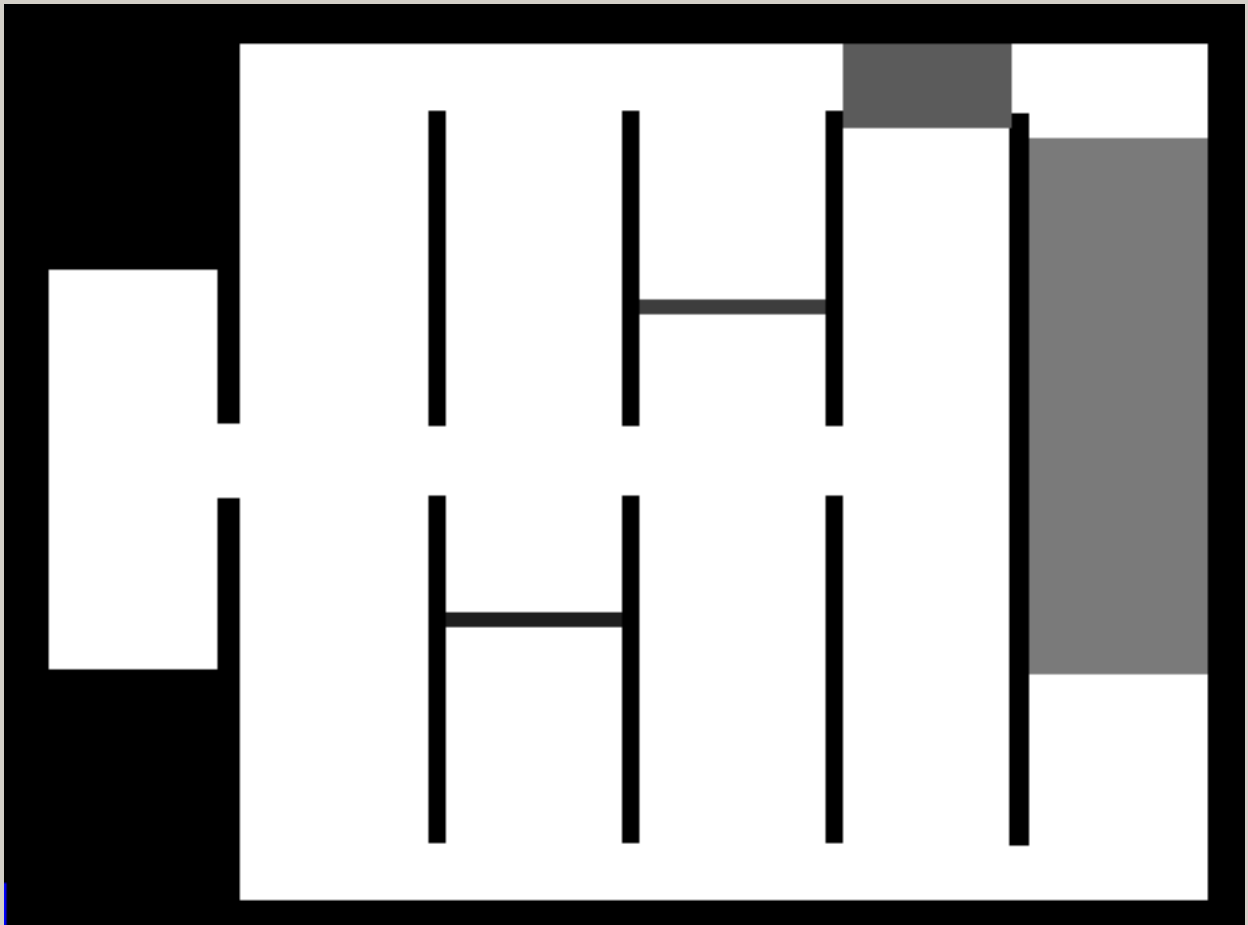
\includegraphics[width=.5\textwidth]{images/stdr_map.png}
				\caption{The map representing the environment where the robot will traverse. Solid black objects represent permanent obstacles while grey obstacles represent temporary obstacles. The darker the obstacle appears, the higher the associated value of $\lambda$. The wait time from time of being observed is given by Eq. (\ref{eqn:waitTime}). The referencing of aisles will be the same as in \S \ref{sec:policySelectionInADynamicEnvironment} with aisles A to E from left to right.}
				\label{fig:stdrMap}
			\end{figure}
			
			This section discusses the implementation of the principles discussed in \S \ref{sec:policySelectionInADynamicEnvironment}. The simulations will be carried out using the STDR Simulator running on Robotics Operating System (ROS). The nodes and all supporting scripts will be coded in python. The map in Fig. \ref{fig:stdrMap} shows the map of the environment that will be used. The map consists of 5 aisles. The start cell and goal cell throughout this section will be the same and al discussions will be for this single case. The start cell is in the bottom of aisle A while the goal cell is in the top of aisle E. The map in Fig. (\ref{fig:stdrMap}) implies that there are 4 temporary obstacles on the map. However only one of them will be active throughout the simulations carried out in this section. This is the obstacle in aisle B.
			\\
			\\
			As we are concerned with comparing the costs of paths down specific aisles, a function needs to be implemented to allow the planning of a path down a chosen aisle. This is accomplished by the \textbf{planPathToGoalViaAisle} method in the \textbf{ReactivePlannerController} class. The method takes 4 parameters of which 1 is optional:
			\begin{itemize}
				\item \textbf{startCellCoords} : The coordinates of the start cell in the search grid (different from the actual coordinates of the cell on the map)
				\item \textbf{goalCellCoords} : The coordinates of the goal cell in the search grid (different from the actual coordinates of the cell on the map)
				\item \textbf{aisle} : The aisle down which a path is desired
				\item \textbf{graphics = True} : Optional parameter that takes a default value of True. Ensures that intermediate searches don't result in constant updating of the search grid graphics. Instead the search grid graphics are only updated during the computation of the path to be traversed by the robot. 
			\end{itemize} 
			
			\begin{figure}[htp]
				\centering
				\begin{subfigure}{.45\textwidth}
					\centering
					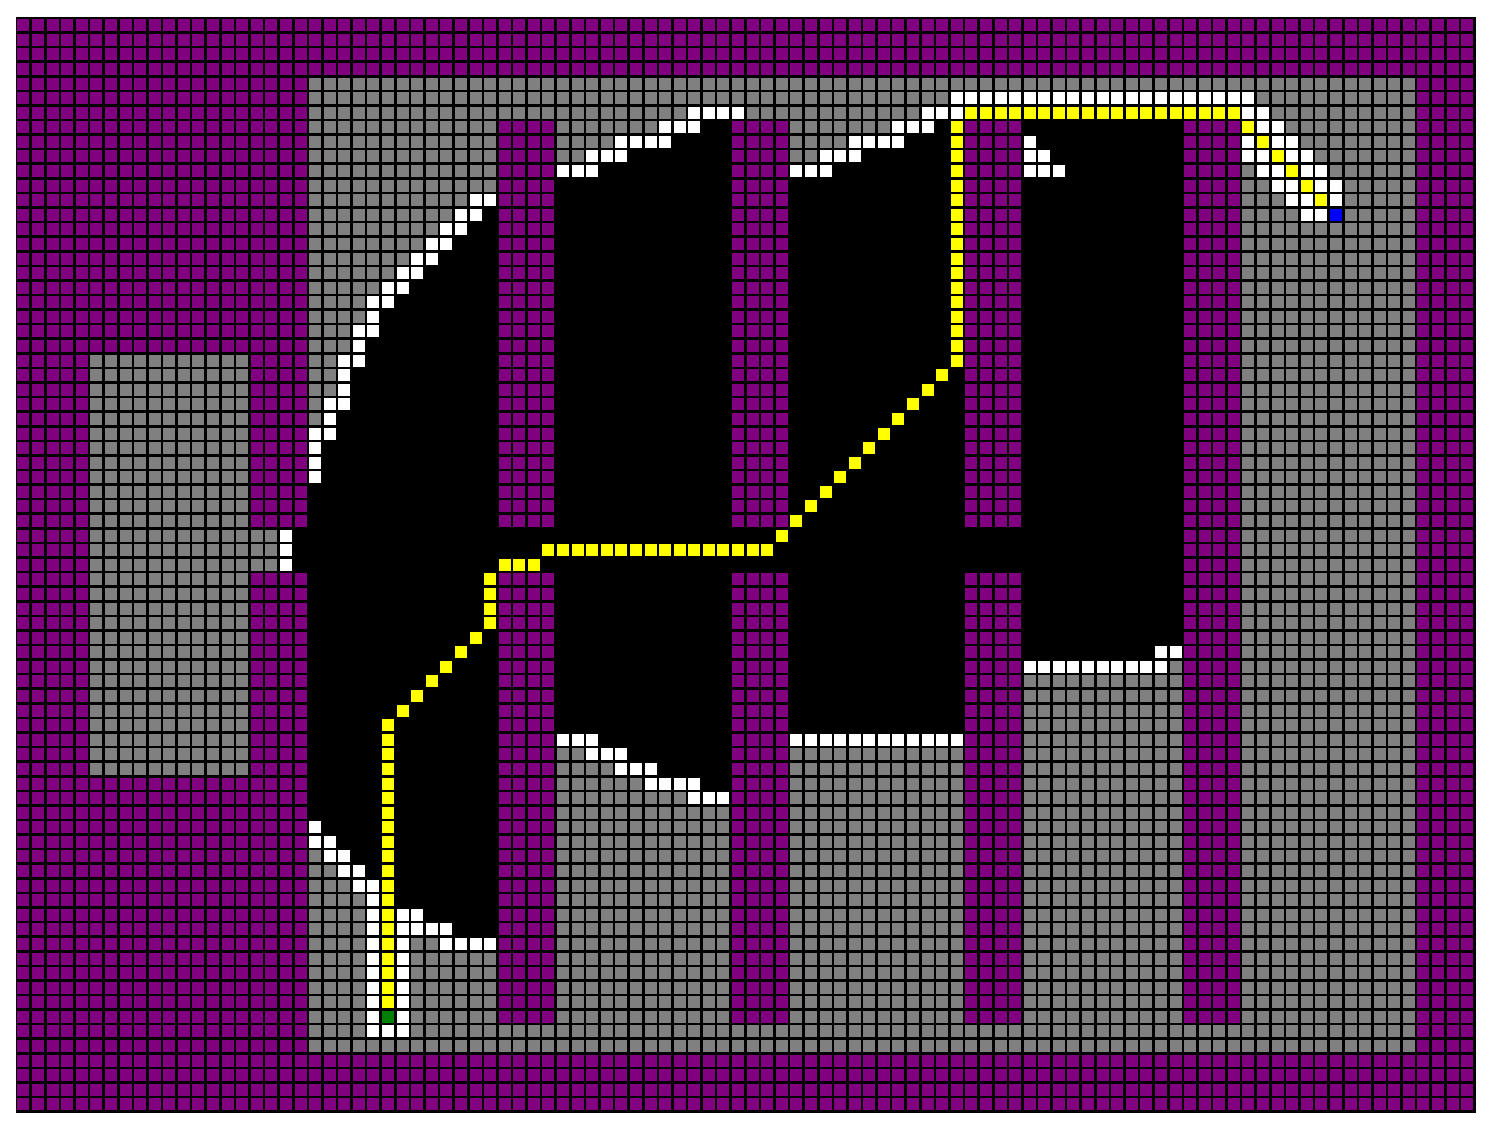
\includegraphics[width=\textwidth]{../exports/initial_search_grid_aisleA}
					\caption{Search grid for a path planned via Aisle A}
					\label{fig:searchGridAisleA}
				\end{subfigure}
				\begin{subfigure}{.45\textwidth}
					\centering
					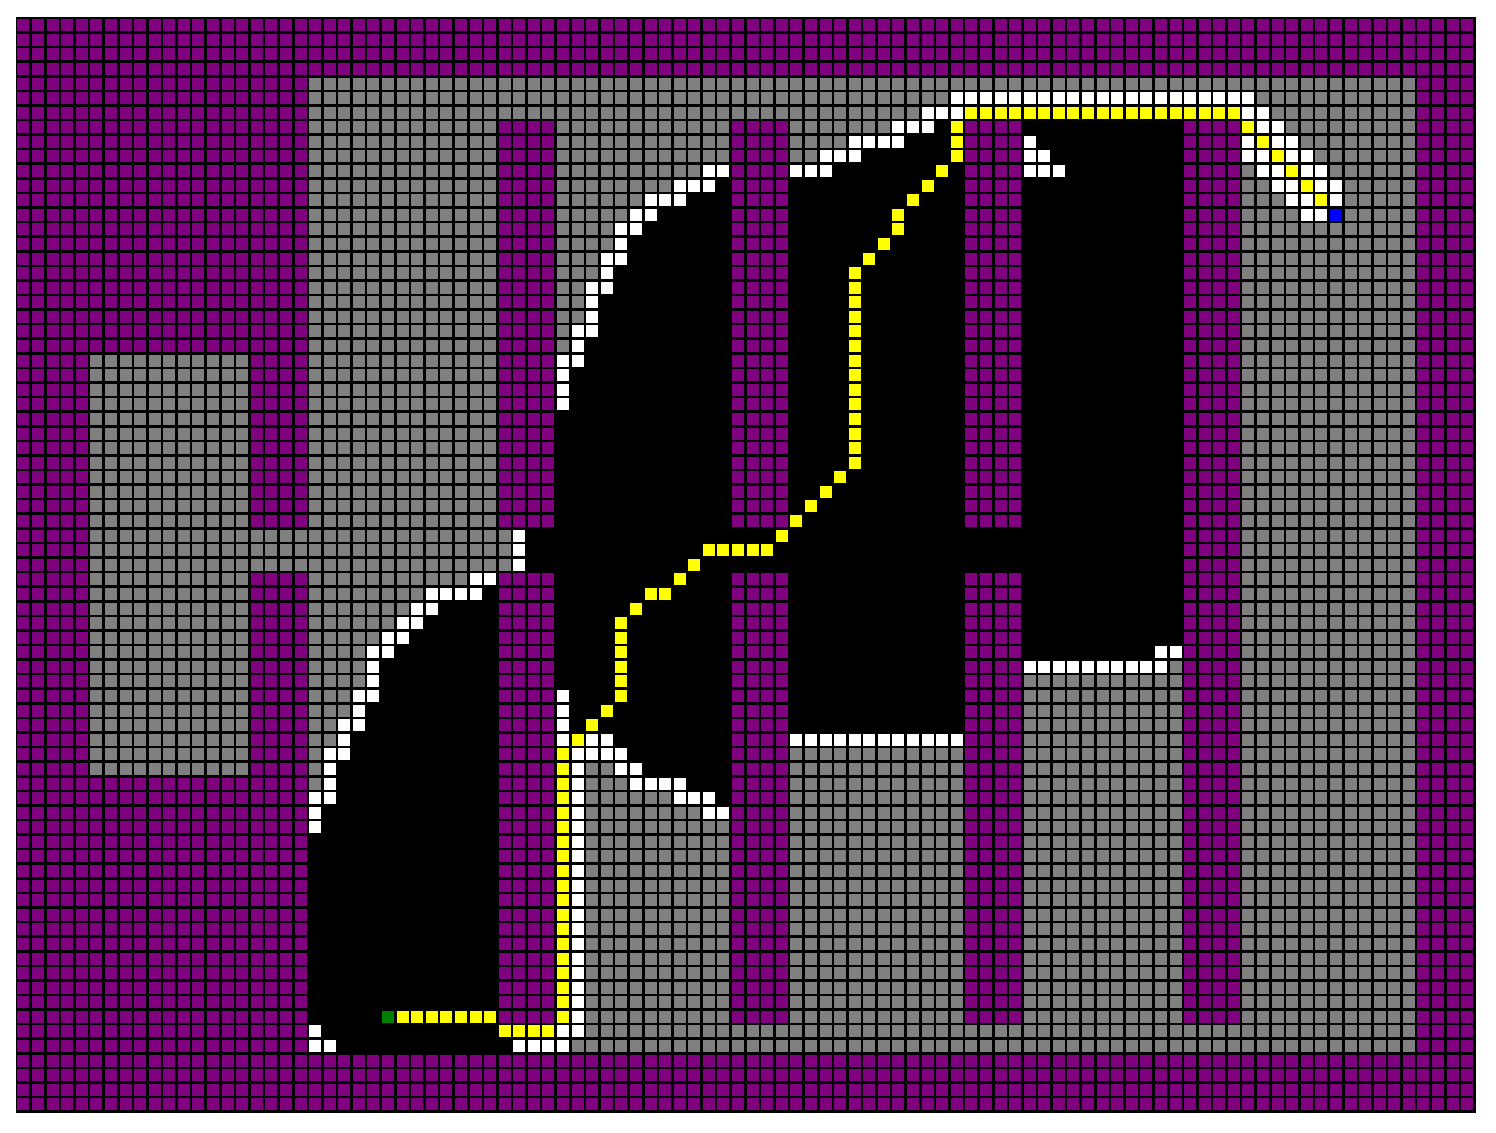
\includegraphics[width=\textwidth]{../exports/initial_search_grid_aisleB}
					\caption{Search grid for a path planned via Aisle B}
					\label{fig:searchGridAisleB}
				\end{subfigure}
				\begin{subfigure}{.45\textwidth}
					\centering
					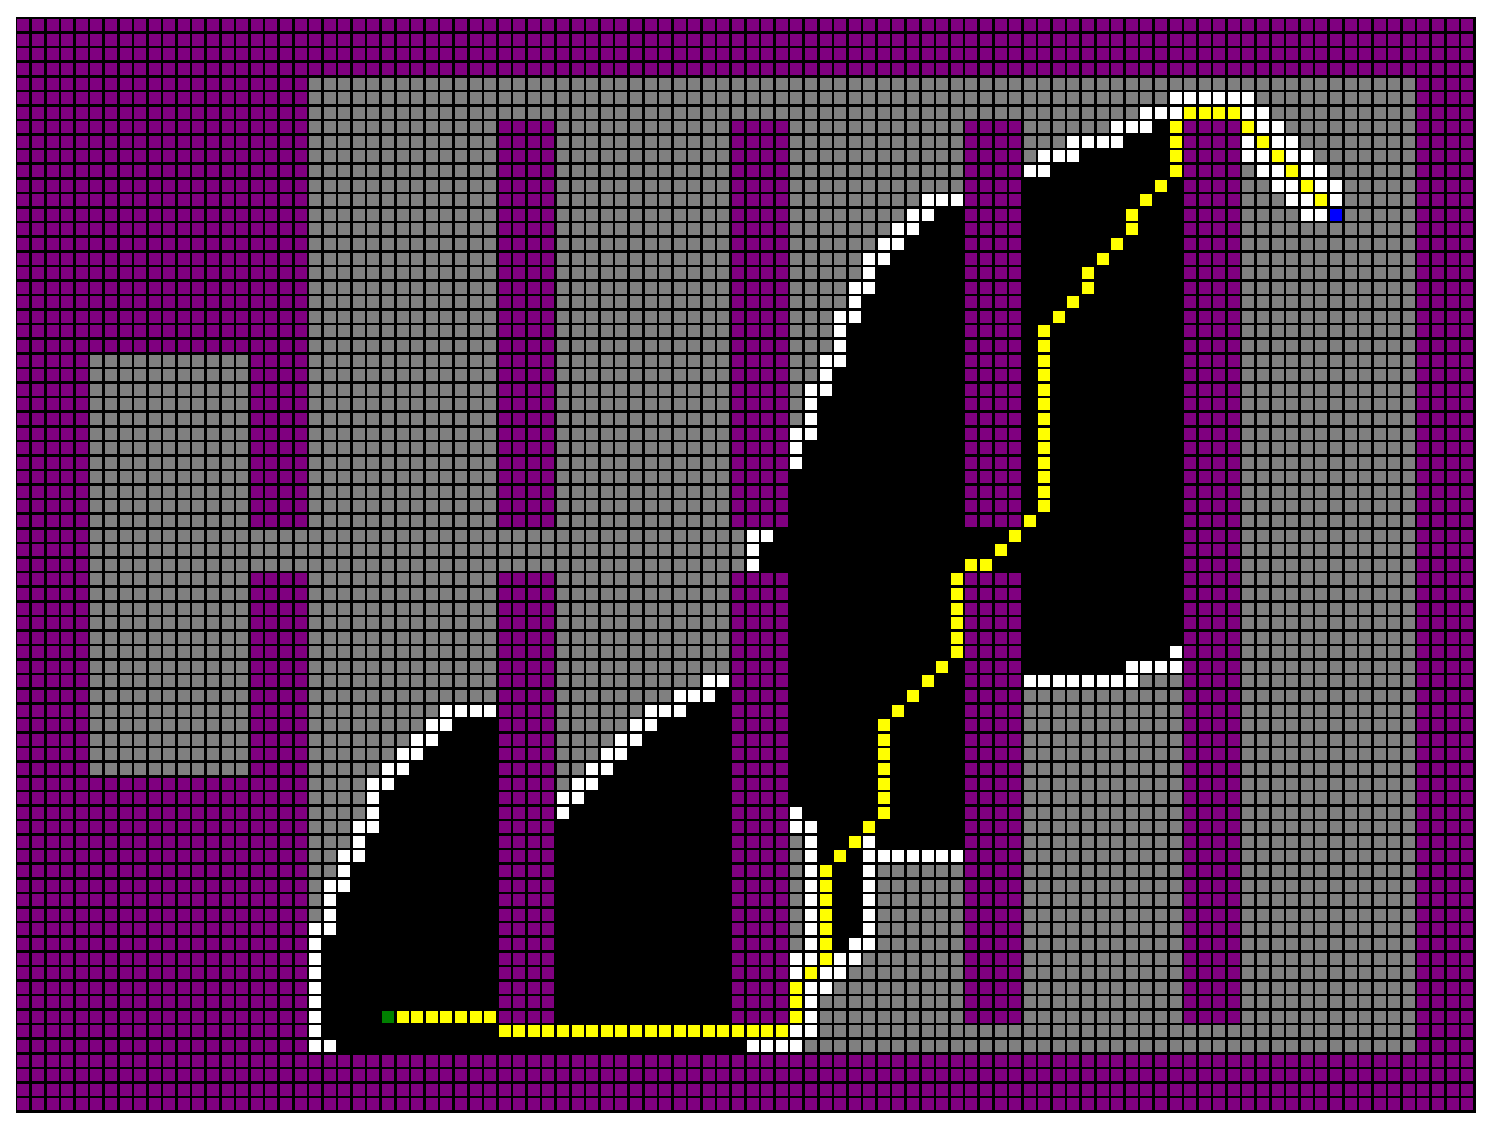
\includegraphics[width=\textwidth]{../exports/initial_search_grid_aisleC}
					\caption{Search grid for a path planned via Aisle C}
					\label{fig:searchGridAisleC}
				\end{subfigure}
				\begin{subfigure}{.45\textwidth}
					\centering
					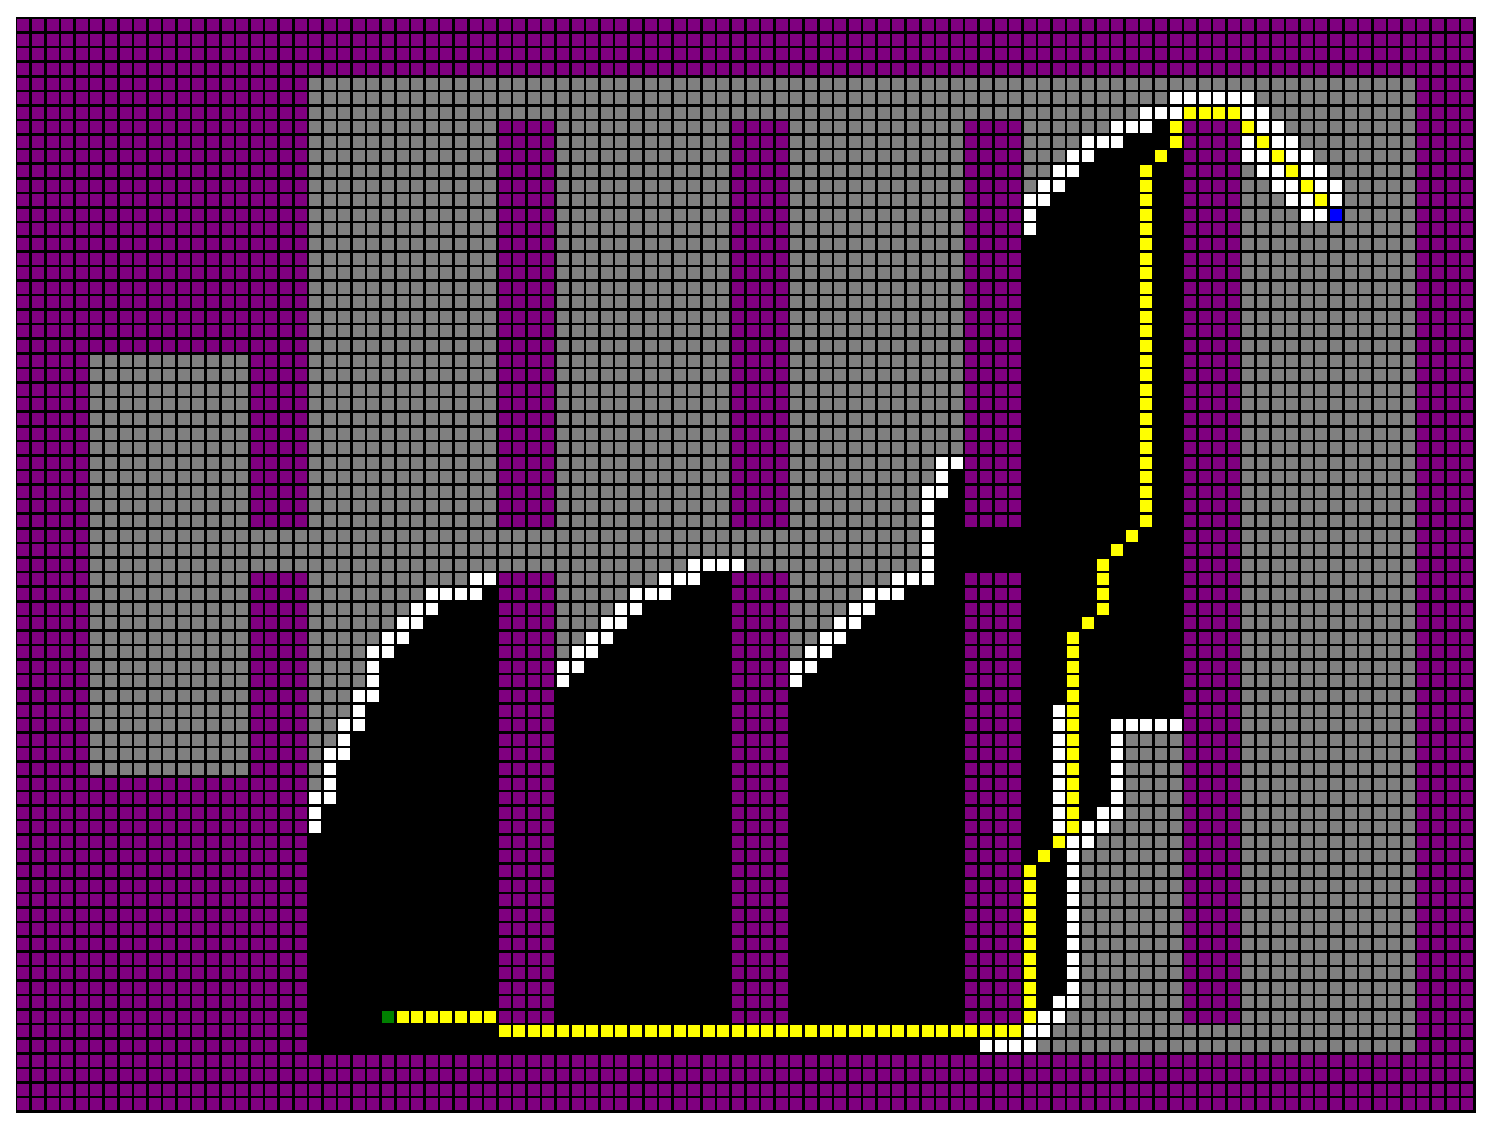
\includegraphics[width=\textwidth]{../exports/initial_search_grid_aisleD}
					\caption{Search grid for a path planned via Aisle D}
					\label{fig:searchGridAisleD}
				\end{subfigure}
				\begin{subfigure}{.45\textwidth}
					\centering
					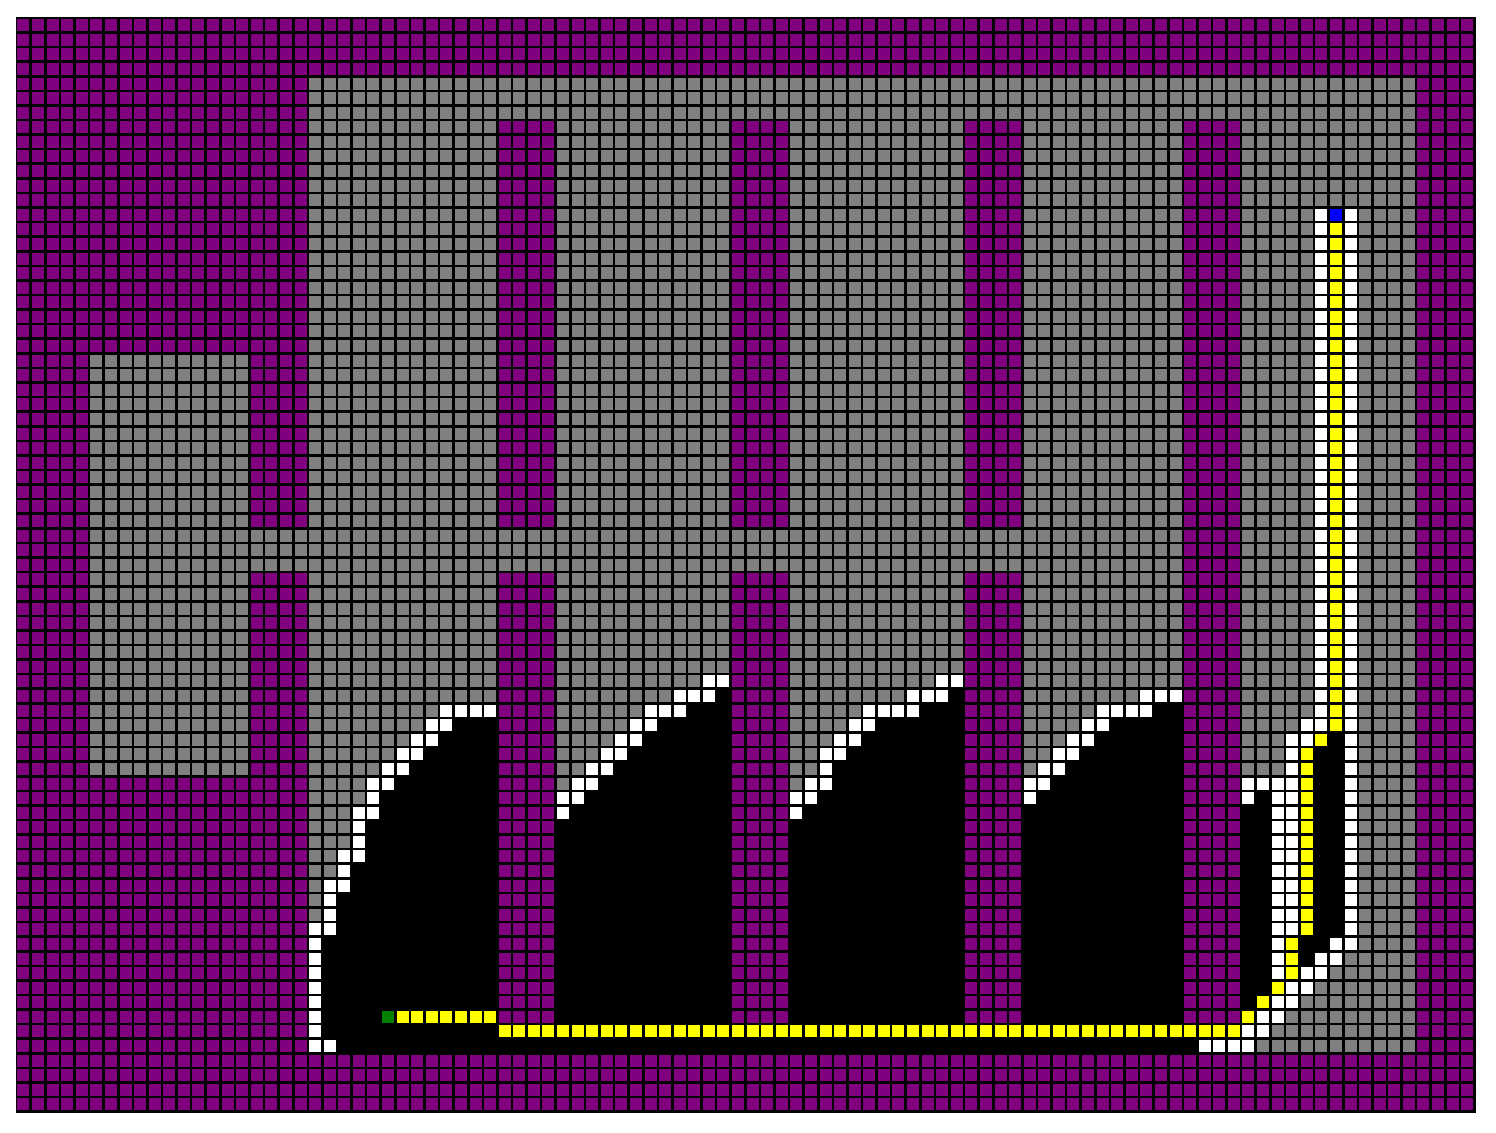
\includegraphics[width=\textwidth]{../exports/initial_search_grid_aisleE}
					\caption{Search grid for a path planned via Aisle E}
					\label{fig:searchGridAisleE}
				\end{subfigure}
				\caption{Search grids for the paths planned from the start (green) to the goal (blue) via a specific aisle. Purple cells indicate obstacles. White cells and Black cells represent alive and dead cells for the search algorithm respectively. Grey cells are unoccupied cells that are unvisited by the search algorithm.}
				\label{fig:searchGridViaAisles}
			\end{figure}
			
			The chosen approach to plan a route down a specific aisle is to split the path planning problem into two parts. In the first part the chosen planner (in this case an A* algorithm with an octile heuristic was implemented by the \textbf{AStarPlanner} class) will plan a path from the start cell (defined by \textbf{startCellCoords})to a cell in the chosen aisle. In the next part the planner will plan a part from the cell in the chosen aisle to the goal cell defined by \textbf{goalCellCoords}. Having obtained these two paths, the next step is to concatenate the two paths to produce the planned path via the chosen aisle. The cells of each aisle are hard coded and returned by a method \textbf{getAisleMidpoint} in the \textbf{ReactivePlannerController} class. The method takes a single parameter which is the chosen aisle. To concatenate the two paths the \textbf{addToEnd} method of the \textbf{PlannedPath} class is used. This method takes a planned path as an argument and adds the waypoints of this planned path to the end of the planned path on which the method is called. It also sums the travel cost and path cardinality.
			\\
			\\
			For the plotting of search grids the two separate search grids from the two executions of the search algorithm need to be merged. This was achieved by the addition of the \textbf{leftMergeGrid} method in the \textbf{SearchGrid} class. This method acts upon a search grid and takes the cell grid of another search grid as a parameter. The search grid taken as the parameter is assumed to be the first search grid corresponding to the path planned from the start to the aisle cell. The start and goal cells are adjusted accordingly and dead/alive are transferred to the latter search grid as well. Finally, the complete planned path was plotted onto the search grid in yellow and then displayed to the user if graphics is enabled. The resulting search grid of paths planned down each aisle is shown Fig. \ref{fig:searchGridViaAisles}. 
		
		\subsection{Waiting for the Obstacle to Clear}
			
			As discussed in \S \ref{sec:policySelectionInADynamicEnvironment}, the robot may choose to wait for an obstacle to clear. During this time the robot should halt it's execution of the current path and wait for the blocking obstacle to clear. This is implemented once again in the \textbf{ReactivePlannerController} class under the \textbf{waitUntilTheObstacleClears} method. This method takes two parameters which are \textbf{startCellCoords} and \textbf{goalCellCoords} (the cell coordinates for the start cell and goal cell respectively). The waiting functionality is achieved by utilizing \textbf{rospy.sleep}. The method checks if the current path is still traversable using the \textbf{checkIfPathCurrentPathIsStillGood} method of the \textbf{ReactivePlannerController} class. While this method returns false, the\textbf{waitUntilTheObstacleClears} method sleeps for 0.5s in simulation time before rechecking. The elapsed wait time is also computed and if the wait time exceeds a set maximum, the robot stop waiting and replans via another aisle chosen by the \textbf{chooseAisle} method. This maximum is defined by the \textbf{maxWaitTime} attribute of the \textbf{ReactivePlannerController} class which in turn is read from the ROS parameter \textbf{max\_wait\_time}.
			\\
			\\
			Once a robot encounters an obstacle it must decide if it is more cost efficient to replan via another aisle or wait for the obstacle to clear so that it can continue on its planned route. This is implemented in the \textbf{ReactivePlannerController} class by the \textbf{shouldWaitUntilTheObstacleClears} method. This method returns true if it is more cost effective to wait and false if the robot should replan. To make a decision on which policy is better, the expected cost of both need to be computed. To compute the cost of replanning we simply call the previously implemented \textbf{planPathToGoalViaAisle} with the desired aisle determined by the \textbf{chooseAisle} method. This returns a \textbf{PlannedPath} object of which the \textbf{travelCost} attribute stores the path cost. To computation of the waiting policy cost is slightly more troublesome. As we do not have access to the obstacle-free map within the \textbf{ReactivePlannerController} class, we need a workaround to compute the path cost of the current cell to the goal cell via the blocked aisle. We do however have access to the planned path that the robot embarked on in the \textbf{currentPlannedPath} attribute. However this includes the section of the path already traversed by the robot. To accommodate for this, a temporary \textbf{AStarPlanner} object was used to plan the path from the current cell to the start cell. By subtracting the cost of this path from the cost of the path stored in \textbf{currentPlannedPath} we obtain the desired path cost.
			\\
			\\
			Finally the expected wait cost needs to be added. This is computed by multiplying the cost of waiting one unit of time ($L_W$) by the expected wait time. The expected wait time is computed by the expression found in Eq. (\ref{eqn:waitTimeExpectation}) and is characterized by the value of $\lambda$. To make a decision as to which policy to choose, the algorithm simply picks the one with the lowest cost: if the cost of waiting is less than the cost of replanning, \textbf{shouldWaitUntilTheObstacleClears} returns true otherwise it returns false. Both the value of $\lambda$ and the value of $L_W$ are read from ROS parameters and can be customized in the launch scripts.
			\\
			\\
			For one instance when the simulation was run, the initially chosen aisle was set to aisle B. When the robot encountered the obstacle, it computed that the path cost of the replanning path was $103.74$ while the path cost of the waiting plan was $98.67$. By considering the expression found in Eq. (\ref{eqn:lambdaInequality}) we can compute the threshold $\lambda$ value under which the robot will always move if it encounters the obstacle. This value is found as shown in Eq. (\ref{eqn:thresholdLambdaReplan}). The cost of waiting one unit of time ($L_W$) is taken to be 2.
			
			\begin{equation}
			\begin{split}
				\lambda_B &\leq \frac{L_W}{PathCost_{Replan} - PathCost_{Wait}} \\
				\lambda_B &\leq \frac{2}{103.74 - 98.67} \\
				\lambda_B &\leq 0.3945
			\end{split}
			\label{eqn:thresholdLambdaReplan}
			\end{equation}
			
		\subsection{Policy Selection at Start}
		
	%%%%%%%%%%%%%%%%%%%%%%%%%%%%%%%%%%%%%%
	\newpage
	\bibliographystyle{IEEEtran}
	\bibliography{references}
	
	%%%%%%%%%%%%%%%%%%%%%%%%%%%%%%%%%%%%%%
	
	\newpage
	\appendix
	\appendixpage
	\addappheadtotoc
	
\end{document}